\documentclass[a4paper, 12pt, margins=2cm]{homework}
\usepackage{tikz}

\usepackage{graphicx}
\usepackage{dsfont}
\usepackage{microtype}
\usepackage{mathrsfs}
\usepackage[ngerman]{babel}
\usepackage{csquotes}
\usepackage[T1]{fontenc}
\usepackage{lmodern}
\usepackage{wasysym}
\usepackage{tabularx}
\usepackage{listings}
\usepackage{algpseudocode}
\usepackage[linesnumbered, lined, boxed, commentsnumbered]{algorithm2e}

\setlength{\parindent}{0pt}

\newcommand{\R}{\mathbb{R}}
\newcommand{\N}{\mathbb{N}}
\newcommand{\Z}{\mathbb{Z}}
\newcommand{\Q}{\mathbb{Q}}
\newcommand{\C}{\mathbb{C}}

\name{Tobias Eidelpes}
\course{Technische Grundlagen der Informatik}
\term{2015WS}
\hwnum{6}
\hwtype{Übungsblatt}
\problemtitle{Aufgabe}
\solutiontitle{Lösung}

\begin{document}

% 1. ERLEDIGT
  \begin{problem}
  \end{problem}
  \begin{solution} \hfill

    \def\svgwidth{1\textwidth}\input{1.pdf_tex}
  \end{solution}

  \begin{problem}
  \end{problem}
  \begin{solution} \hfill
    
    \begin{algorithm}[H]
      \KwResult{Fibonacci with $f_0 = 1$ and $f_1 = 2$}
      
    \end{algorithm}
  \end{solution}


% 3. ERLEDIGT
  \problemnumber{3}
  \begin{problem}
  \end{problem}
  \begin{solution} \hfill
    
    \begin{minipage}{0.5\textwidth}
      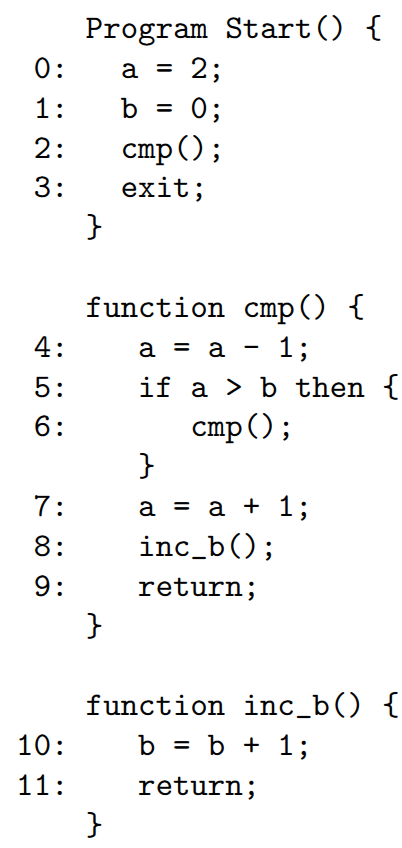
\includegraphics[scale=0.35]{3.png}
    \end{minipage}
    \begin{minipage}{0.5\textwidth}
      \begin{tabular}{|c|c|c|c|c|}
      \hline
        Adresse & a & b & Stack-Operation & Stack-Inhalt \\ \hline \hline
        0       & 2 &   &                 &              \\ \hline
        1       & 2 & 0 &                 &              \\ \hline
        2       & 2 & 0 & push(3)         & 3            \\ \hline
        4       & 1 & 0 &                 &              \\ \hline
        6       & 1 & 0 & push(7)         & 7            \\ \hline
        7       & 2 & 0 &                 &              \\ \hline
        8       & 2 & 0 & push(3)         & 3            \\ \hline
        10      & 2 & 1 &                 &              \\ \hline
      \end{tabular}
    \end{minipage}
    
  \end{solution}

% 4. ERLEDIGT
  \begin{problem}
  \end{problem}
  \begin{solution}\hfill
    
    \begin{center}
      \begin{tabular}{|c|c|c|c|c|}
        \hline
        Befehl & R1 & R2 & R3 & Speicherzugriff(e) \\ \hline
        1      & 0  & 0  & C  & rd(2)              \\ \hline
        2      & A  & 0  & C  &                    \\ \hline
        3      & A  & 5  & C  & rd(C)              \\ \hline
        4      & A  & 5  & 9  & rd(5)              \\ \hline
        5      & 5  & 6  & 8  & rd(6)              \\ \hline
        6      & 5  & 9  & 8  & rd(5), wr(B)       \\ \hline
        7      & 4  & 9  & 8  & wr(4)              \\ \hline
        8      & 4  & 9  & 8  & rd(5), wr(9)       \\ \hline
        9      & 4  & A  & 7  & wr(A)              \\ \hline
        10     & 4  & A  & 7  & wr(A)              \\ \hline
        11     & 4  & 9  & 7  & wr(9)              \\ \hline
        12     & 4  & A  & 7  & rd(0), wr(9)       \\ \hline
        13     & 4  & B  & 7  & wr(3)              \\ \hline
      \end{tabular}
    \end{center}
  \end{solution}

% 5. ERLEDIGT
  \begin{problem}
  \end{problem}
  \begin{solution}\hfill
    
    \begin{enumerate}[label=(\alph*)]\itemsep0pt
      \item Wie lange dauert die Bestückung einer einzelnen Leiterplatte vom Typ PCB3?

            Die Bestückung einer einzelnen PCB3 Leiterplatte dauert 9 Zeiteinheiten.
            \begin{center}
              (3 ZE + 1 ZE + 1 ZE + 3 ZE + 1 ZE) \\ \hfill
            \end{center}
      \item Wie lange dauert es, zehn Leiterplatten vom Typ PCB3 in Folge zu bestücken?

            Zehn Leiterplatten brauchen 42 ZE, weil die erste 15 ZE braucht und jede
            darauffolgende 3 Zeiteinheiten mehr: $15 + 3\cdot 9 = 42$
      \item Wie lange dauert die Bestückung von drei Leiterplatten in der Reihenfolge PCB3–PCB5–PCB4?

            PCB3: 9  ZE (3, 1, 1, 3, 1)\\
            PCB5: 7  ZE (3, 1, 1, 1, 1)\\
            PCB4: 10 ZE (1, 1, 2, 3, 3)\\

            $7\cdot 3 = 21$ Zeiteinheiten

      \item Kann die Gesamtdauer aus Teilaufgabe c) durch Umordnung der Reihenfolge verkürzt werden?

            Ja, indem man beispielsweise die Leiterplatte vom Typ PCB4 an den Anfang stellt.
    \end{enumerate}
  \end{solution}

% 7. ERLEDIGT
  \problemnumber{7}
  \begin{problem}
  \end{problem}
  \begin{solution}\hfill
    
    \begin{enumerate}[label=(\alph*)]\itemsep0pt
      \item \hfill
        \begin{center}
          \begin{tabular}{|c||c|c|c|c|}
            \hline
            Zeit $\downarrow$ & F    & D    & E    & S    \\ \hline \hline
            1    & ADD  &      &      &      \\ \hline
            2    & PUSH & ADD  &      &      \\ \hline
            3    & OR   & PUSH & ADD  &      \\ \hline
            4    & AND  & OR   & PUSH & ADD  \\ \hline
            5    & AND  & OR   &      & PUSH \\ \hline
            6    & DIV  & AND  & OR   &      \\ \hline
            7    & POP  & DIV  & AND  & OR   \\ \hline
            8    & POP  & DIV  &      & AND  \\ \hline
            9    &      & POP  & DIV  &      \\ \hline
            10   &      &      & POP  & DIV  \\ \hline
            11   &      &      &      & POP  \\ \hline
         \end{tabular}
        \end{center}

      \item \hfill

      \centering\def\svgwidth{0.8\textwidth}\input{7b.pdf_tex}
    \end{enumerate}
  \end{solution}


\end{document}